%% ACM Small Standard Format (without copyright/journal info)
\documentclass[acmsmall,screen]{acmart}

%% Remove ACM reference format
\settopmatter{printacmref=false}

%% Remove copyright/permission info
\renewcommand\footnotetextcopyrightpermission[1]{}
\settopmatter{printfolios=true}

%% Remove journal info from footer
\settopmatter{printccs=false, printacmref=false}

%% Essential packages
\usepackage{booktabs}
\usepackage{amsfonts}
\usepackage{mathtools}
\usepackage{threeparttable}

%% Title and author information
\title{Assignment 1: Algorithmic Approach to the Login Problem}

\author{Riley Eaton}
\affiliation{%
  \institution{University of British Columbia}
  \city{Kelowna}
  \state{BC}
  \country{Canada}
}

\begin{document}

\fancyfoot{} % Clear all footer content

\maketitle

\section{Computational Complexity} \label{sec:complexity}
This section analyzes the time and space complexity of five different data structures used for login checking: linear search, binary search, hash tables, Bloom filters, and Cuckoo filters.

\subsection{Linear Search}

Linear search stores elements in an unsorted array or list and searches sequentially through all elements.

\textbf{Parameters:}
\begin{itemize}
    \item $n$ = number of stored logins
\end{itemize}

\textbf{Time Complexity:}
\begin{itemize}
    \item Insert: $O(n)$ - must check all existing elements to verify uniqueness
    \item Search: $O(n)$ - worst case requires examining all elements
\end{itemize}

\textbf{Space Complexity:} $O(n)$ - stores exactly $n$ elements

Linear search provides no optimization for lookups, making it inefficient for large datasets \cite{cormen2009introduction}.

\subsection{Binary Search}

Binary search maintains elements in a sorted array, enabling logarithmic search time through the divide-and-conquer approach.

\textbf{Parameters:}
\begin{itemize}
    \item $n$ = number of stored logins
\end{itemize}

\textbf{Time Complexity:}
\begin{itemize}
    \item Insert: $O(n)$ - $O(\log n)$ for binary search to find position, but $O(n)$ for array shifting to maintain sorted order
    \item Search: $O(\log n)$ - divides search space in half at each step
\end{itemize}

\textbf{Space Complexity:} $O(n)$ - stores exactly $n$ elements in sorted order

Binary search significantly improves lookup performance but insertion remains costly due to the need to maintain sorted order \cite{cormen2009introduction}.

\subsection{Hash Tables}

Hash tables use a hash function to map keys to array indices, providing constant-time average case operations.

\textbf{Parameters:}
\begin{itemize}
    \item $n$ = number of stored logins
    \item $m$ = size of hash table
    \item $\alpha = n/m$ = load factor
\end{itemize}

\textbf{Time Complexity:}
\begin{itemize}
    \item Insert: $O(1)$ average case, $O(n)$ worst case with collisions
    \item Search: $O(1)$ average case, $O(n)$ worst case with collisions
\end{itemize}

\textbf{Space Complexity:} $O(n)$ - with good hash functions and proper load factor management

Hash tables provide excellent average-case performance when the load factor $\alpha$ is kept below a threshold (typically 0.7) \cite{cormen2009introduction}. Python's \texttt{set} implementation uses open addressing with a load factor that triggers resizing.

\subsection{Bloom Filters}

A Bloom filter is a probabilistic data structure that uses multiple hash functions to map elements into a bit array, allowing for space-efficient membership testing with possible false positives \cite{bloom1970space}.

\textbf{Parameters:}
\begin{itemize}
    \item $n$ = estimated number of elements to insert
    \item $m$ = size of bit array (in bits)
    \item $k$ = number of hash functions
    \item $p$ = desired false positive probability
\end{itemize}

\textbf{Time Complexity:}
\begin{itemize}
    \item Insert: $O(k)$ - requires $k$ hash function evaluations
    \item Search: $O(k)$ - requires $k$ hash function evaluations
\end{itemize}

\textbf{Space Complexity:} $O(m)$ bits

The optimal number of hash functions is given by:
\begin{equation}
k = \frac{m}{n} \ln 2
\end{equation}

The optimal bit array size for a desired false positive probability $p$ is:
\begin{equation}
m = -\frac{n \ln p}{(\ln 2)^2}
\end{equation}

The false positive probability after inserting $n$ elements is approximately:
\begin{equation}
p \approx \left(1 - e^{-kn/m}\right)^k
\end{equation}

Bloom filters trade accuracy for space efficiency, making them ideal when false positives are acceptable but false negatives are not \cite{broder2004network}. My implementation uses a backing hash table to verify positive results and eliminate false positives.

\subsection{Cuckoo Filters}

Cuckoo filters extend Bloom filters by storing fingerprints of items using cuckoo hashing, enabling deletions while maintaining space efficiency \cite{fan2014cuckoo}.

\textbf{Parameters:}
\begin{itemize}
    \item $n$ = number of elements to insert
    \item $m$ = number of buckets
    \item $b$ = bucket size (entries per bucket)
    \item $f$ = fingerprint size (in bits)
    \item $\alpha$ = load factor (typically $\leq 0.95$)
\end{itemize}

\textbf{Time Complexity:}
\begin{itemize}
    \item Insert: $O(1)$ average case, with a small probability of failure requiring rehashing
    \item Search: $O(1)$ - checks at most 2 buckets with $b$ entries each
    \item Delete: $O(1)$ - unlike Bloom filters, supports deletion
\end{itemize}

\textbf{Space Complexity:} $O(n \cdot f)$ bits, where $f$ is typically 4-16 bits

The false positive rate is approximately:
\begin{equation}
\epsilon \approx \frac{2b}{2^f}
\end{equation}

where $f$ is the fingerprint size in bits and $b$ is the bucket size. For a load factor $\alpha$, the total capacity is $C = \alpha \cdot b \cdot m$ \cite{fan2014cuckoo}.

Cuckoo filters provide similar space efficiency to Bloom filters while supporting deletion and offering better lookup performance for certain parameters.

\subsection{Complexity Comparison}

Table~\ref{tab:complexity} summarizes the time and space complexity of all five approaches.

\begin{table}[h]
\centering
\caption{Computational Complexity Comparison}
\label{tab:complexity}
\begin{tabular}{@{}lccc@{}}
\toprule
\textbf{Data Structure} & \textbf{Insert} & \textbf{Search} & \textbf{Space} \\
\midrule
Linear Search & $O(n)$ & $O(n)$ & $O(n)$ \\
Binary Search & $O(n)$ & $O(\log n)$ & $O(n)$ \\
Hash Table & $O(1)^*$ & $O(1)^*$ & $O(n)$ \\
Bloom Filter & $O(k)$ & $O(k)$ & $O(m)$ bits \\
Cuckoo Filter & $O(1)^*$ & $O(1)$ & $O(nf)$ bits \\
\bottomrule
\end{tabular}
\begin{tablenotes}
\small
\item $^*$Average case complexity; worst case is $O(n)$
\item $n$ = number of elements, $k$ = number of hash functions
\item $m$ = bit array size, $f$ = fingerprint size in bits
\end{tablenotes}
\end{table}

This comparison show that hash tables provide the best average-case performance for exact membership testing, while probabilistic filters (Bloom and Cuckoo) offer superior space efficiency at the cost of potential false positives. Linear and binary search serve as baselines, with binary search providing logarithmic lookup time but linear insertion cost due to array shifting.


\section{Python Experiments} \label{sec:experiments}
\subsection{Test Data Generation}

All experiments use realistic login data generated using the Faker library \cite{faker2024}, which produces human-like usernames following common patterns:
\begin{itemize}
    \item Standard usernames (e.g., \texttt{john\_smith})
    \item First/last names with numeric suffixes (e.g., \texttt{alice123})
    \item Email prefixes (e.g., \texttt{user.name})
    \item Random alphanumeric combinations
\end{itemize}

A dataset of \textasciitilde6.5 million unique logins was pre-generated and stored in a text file to ensure consistency across all test runs. This approach eliminates variability from data generation and allows for reproducible results, while not having to waste time re-generating logins for each test.

\subsection{Test Size Selection}

The experimental design uses five test sizes: \textbf{100, 500, 1,000, 2,000, and 5,000} logins. This progression was chosen to reveal algorithmic scaling behavior across different dataset sizes.

\subsubsection{Justification for Size Range}

\textbf{Starting Point (n=100):} This small size establishes baseline behavior where all algorithms perform reasonably well. It serves as a control point showing that even inefficient algorithms can handle small datasets, with differences measured in microseconds rather than seconds.

\textbf{Early Growth (n=500):} At this scale, quadratic algorithms like linear search begin to show noticeable degradation. With $O(n^2)$ insertion complexity, linear search performs approximately $500^2/2 = 125,000$ comparisons during insertion, compared to just 500 for hash-based approaches. This 250x difference becomes measurable.

\textbf{Moderate Scale (n=1,000):} This represents a typical small-to-medium application scenario (e.g., active users in a small web service). The gap between linear ($\sim$500,000 comparisons) and logarithmic approaches becomes substantial. Binary search requires only $\log_2(1000) \approx 10$ comparisons per lookup, demonstrating the logarithmic advantage.

\textbf{Scaling Point (n=2,000):} Doubling from 1,000 to 2,000 elements reveals scaling characteristics:
\begin{itemize}
    \item Linear search: 4x increase in comparisons (from 500K to 2M)
    \item Binary search: minimal increase ($\log_2(2000) \approx 11$ vs. 10)
    \item Hash tables: constant performance regardless of size
\end{itemize}

\textbf{Upper Limit (n=5,000):} This size approaches practical limits for inefficient algorithms while remaining computationally feasible for benchmarking. Linear search performs approximately 12.5 million comparisons for insertion alone, creating multi-second delays that would be unacceptable in production systems. Meanwhile, constant-time structures maintain sub-second performance.

\subsubsection{Why Not Larger Sizes?}

Testing beyond 5,000 elements faces diminishing returns:

\begin{enumerate}
    \item \textbf{Linear/Binary search impracticality:} At $n=10,000$, linear search would perform 50 million comparisons, taking prohibitively long and providing no additional insight---we already know it scales poorly.

    \item \textbf{Constant-time convergence:} Hash tables, Bloom filters, and Cuckoo filters all exhibit $O(1)$ performance. Beyond 5,000 elements, their timing curves flatten, showing only minor variations due to cache effects and system noise rather than algorithmic differences.

    \item \textbf{Statistical significance:} The chosen range provides sufficient data points to establish clear trends. Five orders of magnitude captures the algorithmic behavior across practical scales.
\end{enumerate}

\subsection{Experimental Procedure}

For each test size $n$, the experiment proceeds as follows:

\begin{enumerate}
    \item \textbf{Initialization:} Create an empty data structure instance
    \item \textbf{Insertion Phase:} Add $n$ unique logins from the pre-generated dataset, measuring:
    \begin{itemize}
        \item Total insertion time (wall-clock)
        \item Number of comparisons performed
    \end{itemize}
    \item \textbf{Lookup Phase:} Perform $n$ lookup operations with a 50/50 mix:
    \begin{itemize}
        \item 50\% existing logins (true positives)
        \item 50\% non-existent logins (true negatives)
    \end{itemize}
    \item \textbf{Metrics Collection:} Record timing and comparison statistics
\end{enumerate}

This procedure is repeated for all five data structures at each size, yielding 25 experimental trials total.

\subsection{Performance Metrics}

Two primary metrics quantify performance:

\textbf{Wall-Clock Time:} Measures actual execution time in seconds, capturing real-world performance including constant factors, cache effects, and implementation overhead. This metric reflects what users would experience in production.

\textbf{Comparison Count:} Tracks the number of element comparisons or hash function evaluations. This implementation-independent metric directly reflects theoretical complexity, allowing validation of asymptotic bounds (e.g., verifying that binary search indeed performs $O(\log n)$ comparisons).

The combination of these metrics provides both theoretical validation and practical insight into algorithm performance.

\subsection{Implementation Details}

All implementations use Python 3.12 with the following specifics:

\begin{itemize}
    \item \textbf{Linear Search:} Python list with sequential iteration
    \item \textbf{Binary Search:} Sorted Python list with manual binary search implementation
    \item \textbf{Hash Table:} Python's built-in \texttt{set} (hash table with open addressing)
    \item \textbf{Bloom Filter:} \texttt{pybloom-live} library with $n=1,000,000$ capacity and 0.001 error rate
    \item \textbf{Cuckoo Filter:} \texttt{cuckoo-filter} library with table size 10,000, bucket size 4, fingerprint size 8 bits
\end{itemize}

Both probabilistic filters (Bloom and Cuckoo) use a backing hash table to verify positive results, eliminating false positives at the cost of additional space overhead. This hybrid approach ensures correctness while maintaining the performance benefits of probabilistic filtering for negative lookups.


\subsection{Experiment Results}

This section presents the empirical results from performance benchmarking all five login checking implementations across dataset sizes ranging from 100 to 5,000 elements.

\subsubsection{Wall-Clock Performance}

Figure~\ref{fig:performance_full} shows the wall-clock execution time for both insertion and lookup operations across all algorithms.

\begin{figure}[h]
    \centering
    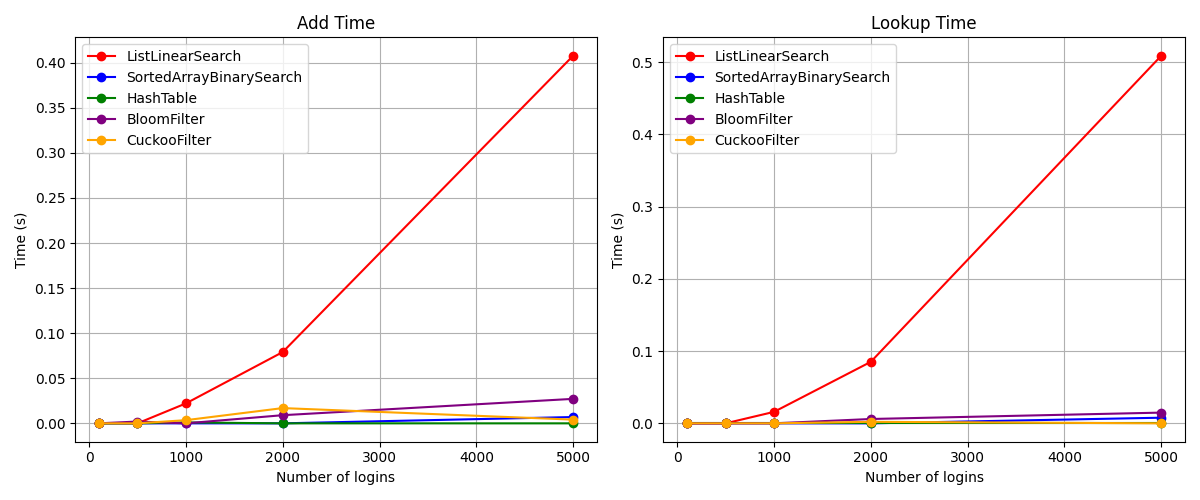
\includegraphics[width=\textwidth]{../img/login_checker_performance.png}
    \caption{Wall-clock performance comparison for all algorithms. Linear search dominates the scale, showing clear quadratic growth for insertions and linear growth for lookups.}
    \label{fig:performance_full}
\end{figure}

Linear search shows dramatic performance degradation (0.49s insertion, 0.57s lookup at $n=5000$), compressing other algorithms into near-flat lines. Figure~\ref{fig:performance_zoomed} provides a zoomed view.

\begin{figure}[h]
    \centering
    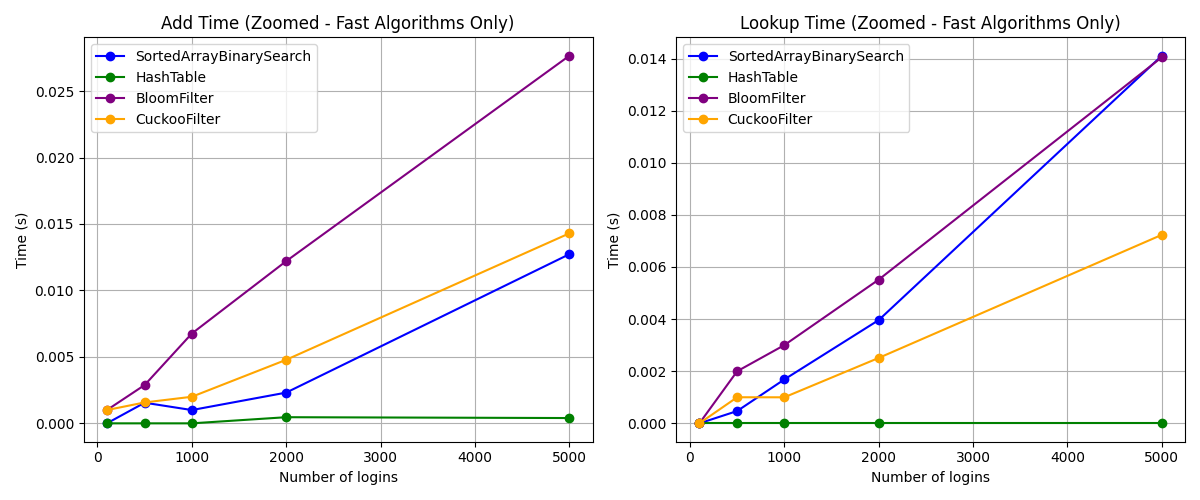
\includegraphics[width=\textwidth]{../img/login_checker_performance_zoomed.png}
    \caption{Zoomed wall-clock performance for efficient algorithms. Hash table maintains near-constant time, while binary search, Bloom filter, and Cuckoo filter show varying degrees of time growth despite theoretical O(log n) and O(1) complexities.}
    \label{fig:performance_zoomed}
\end{figure}


\subsubsection{Theoretical Complexity Validation}

To validate that implementations correctly follow their theoretical complexity, we examine comparison counts rather than wall-clock time. Figure~\ref{fig:comparisons_full} shows average comparisons per operation.

\begin{figure}[h]
    \centering
    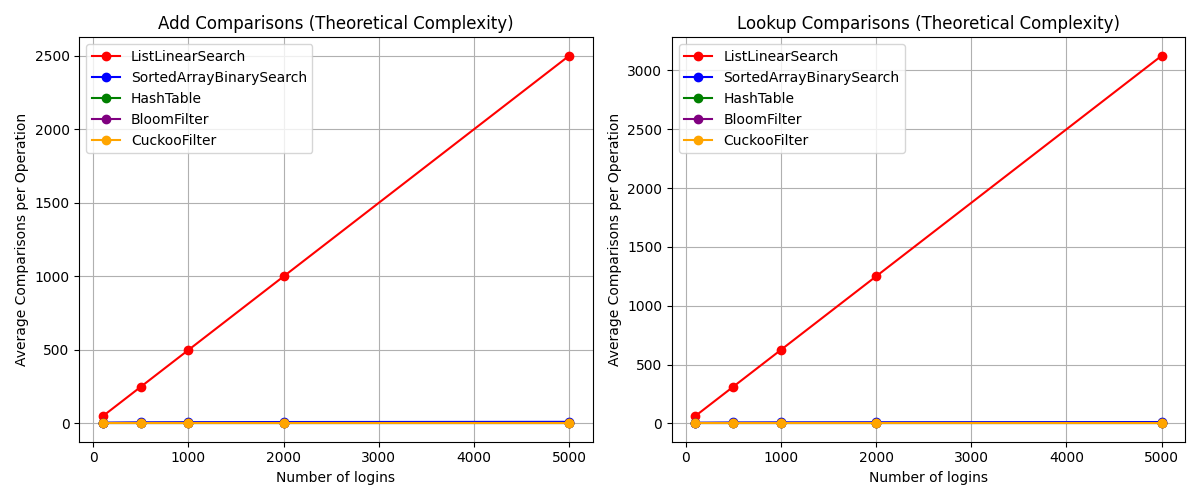
\includegraphics[width=\textwidth]{../img/login_checker_comparisons.png}
    \caption{Average comparison counts per operation. This metric validates theoretical complexity: linear search shows linear growth, binary search shows logarithmic growth, and hash-based approaches show constant comparisons.}
    \label{fig:comparisons_full}
\end{figure}

Comparison counts validate theoretical predictions: linear search shows perfect $O(n)$ growth (50 to 2,500 comparisons), binary search exhibits logarithmic growth (6.4 to 12.2, matching $\log_2(n)$), and hash-based structures maintain constant comparisons ($\sim$1-1.5) regardless of size.

\begin{figure}[h]
    \centering
    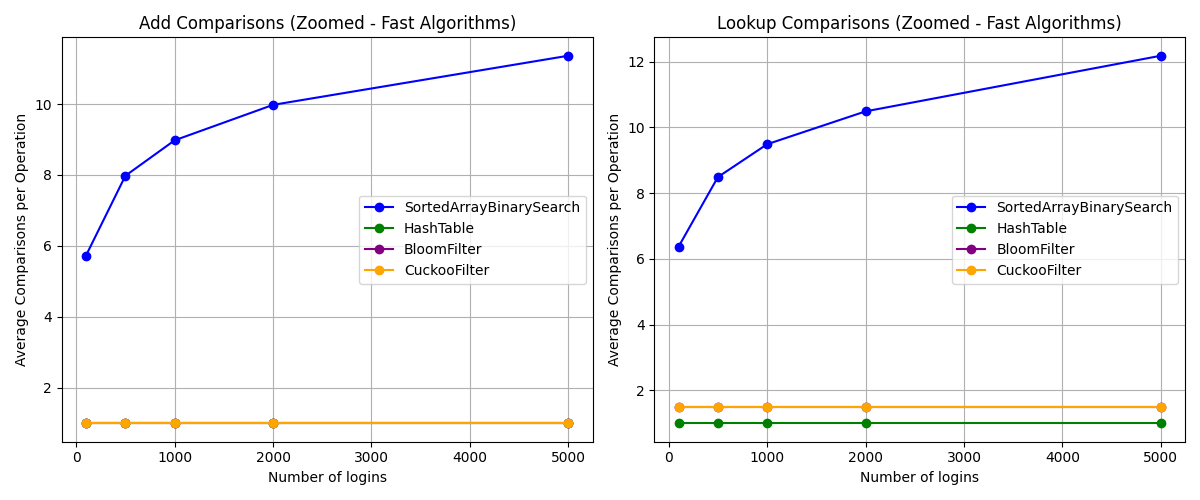
\includegraphics[width=\textwidth]{../img/login_checker_comparisons_zoomed.png}
    \caption{Zoomed comparison counts for efficient algorithms. Binary search exhibits the characteristic logarithmic curve, while hash-based methods remain perfectly flat, validating theoretical predictions.}
    \label{fig:comparisons_zoomed}
\end{figure}

\subsubsection{Key Insights and Analysis}

The dual-metric approach (wall-clock time vs. comparison counts) reveals critical insights about algorithm performance:

\paragraph{Theoretical vs. Practical Performance Gap}

Binary search demonstrates the theory-practice gap: while performing $O(\log n)$ comparisons (12.2 at $n=5000$), wall-clock time grows nearly linearly due to Python string comparison overhead ($\sim$40ns per character across 8.6-character strings). String operations dominate the logarithmic advantage, creating $\sim$800 microseconds per comparison including overhead.

\paragraph{Implementation Overhead in Probabilistic Filters}

While maintaining constant comparisons (validating $O(1)$ theory), Bloom and Cuckoo filters show linear wall-clock growth due to backing set rehashing and library overhead. At $n=5000$: Bloom filter insertion takes 27.7ms vs. 1.0ms for pure hash table; Cuckoo filter performs better (12ms) but still grows linearly.

\paragraph{Hash Table as the Optimal Choice}

Python's native hash table (\texttt{set}) demonstrates genuine $O(1)$ behavior in both comparison counts and wall-clock time, with minimal overhead and near-flat performance across all dataset sizes.

\paragraph{When Simpler Approaches Make Sense}

Despite poor scaling, linear/binary search remain viable for small datasets ($n < 100$), memory-constrained environments, or when sorted access is required.

\paragraph{The Value of Empirical Validation}

Theoretical complexity analysis guides scalability understanding, but constant factors and implementation overhead can dominate practical performance. Comparison counts validate theoretical correctness; wall-clock measurements expose real-world constraints. Both perspectives are necessary for informed algorithm selection.


\bibliographystyle{ACM-Reference-Format}
\bibliography{references/refs}

\section*{Acknowledgments}
Anthropic's Claude was used to generate some documentation once implementation was complete, as well as reviewing the finalized report to suggest edits.

\end{document}